\documentclass[eprint]{actapoly}

\begin{document}

\title[Implementation of the INSPIRE Theme Buildings]
{Analysis and Implementation of Application Schemas for the INSPIRE Theme Buildings}

%\correspondingauthor[M. Med]{michal Med}{my}{my@mail.com}
\correspondingauthor[M. Med]{Michal Med}{my}{michal.med@fsv.cvut.cz}

\institution{my}{Faculty of Civil Engineering, Czech Technical University in Prague, Thakurova 2077/7, Prague, Czech Republic}
%\institution{their}{Their institution, Their Road 1, Their Town, Their Country}

\begin{abstract}
During the Implementation of INSPIRE directive, various data themes are transformed into structure and content given by Data Specifications published by Joint Research Center of the European Commission. Data shall be published in the GML format, that is standard of Open Geospatial Consortium. Validity of data structure is ensured by validation against XSD schemas. These schemas are usually provided by JRC as well, but not necessarily for all application schemas.

Currently implemented theme Buildings has defined six application schemas, but XSD schemas are available for only three of them. All application schemas were analysed and it was found, that the most suitable data model responds most closely to the application schema BuildingsExtended2D. Its XSD schema was not provided by JRC in the current version. Moreover, abstract XSD schema BuildingsExtendedBase, needed for usage of previous schemas, neither. There appeared a need of creation of these missing XSD schemas.

%Besides suitable application schema, analysis showed data sources needed for implementation, presumed links to features of other INSPIRE themes, default portrayal and ways of data publication. During implementation, data were transformed from original databases into tables in publication database, then it was shaped into INSPIRE data structure given by Data Specification and published in GML format, valid against newly created XSD schemas.
\end{abstract}

\keywords{INSPIRE, Buildings, XSD schema, GML format, web service}

\maketitle




\section{Introduction to INSPIRE}
Infrastructure for Spatial Information in Europe (INSPIRE) is the directive of European Commission and Council, which was created to standardise spatial information in member countries of EU and enable the sharing of information among public sector organisations. Its implementation has begun on 15th May 2007 by coming Directive 2007/2/EC of the European Parliament and Council into force. Interoperability of spatial data sets and services is ensured by Commission Regulation No 1089/2010 of 23rd November 2010. This regulation was amended by Commission Regulations 102/2011 of 4th February 2011 and 1253/2013 of 21st October 2013. Directive is planned to be implemented at various stages, with full implementation required by 2019. In the Czech Republic it was transposed into legislation by the amendment to the Act no. 123/1998 Coll., on the right to access information about environment, which came into force on 23rd October 2009. 

\begin{figure}
\centering
\includegraphics[width=0.8\linewidth]{pics/inspire_logo.png} % <-- use this for your graphics
%\rule{10cm}{5cm} % <-- this is just a black box substitute for graphics
\caption{Logo of the INSPIRE project.}
\label{fig:inspire_logo}
\end{figure}

Joint Research Center has no legal right to push national mapping agencies into publishing INSPIRE--compliant data, metadata and services. For this purpose, national coordinating body was founded in every participating country. Coordination is ensured on the national level. Implementation of INSPIRE is in Czech Republic coordinated by Czech information agency of environment (CENIA). On 4th November 2010 was found Coordinating Committee for INSPIRE (KOVIN) as an advisory body of the Ministry of environment. Its tasks are the implementation of INSPIRE, evaluating progress in promoting the implementation of INSPIRE, analysis of results of the implementation and coordination of data providers. This is done through technical working groups focused on partial implementation steps, such as metadata, services, strategy, legislation i.e.
\cite{KOVIN}

\begin{figure*}
\centering
\includegraphics[width=0.8\linewidth]{pics/feature_catalogue.png} % <-- use this for your graphics
%\rule{10cm}{5cm} % <-- this is just a black box substitute for graphics
\caption{Example of the feature catalogue for the spatial object Building.}
\label{fig:feature_catalogue}
\end{figure*}

Since the beginning of 2014, the implementation is documented and directed by the national strategy of the implementation of INSPIRE \cite{strategie}. Main target of the implementaion according to the strategy is creation, maintenance and developing of the infrastructure of spatial information in the Czech Republic as a part of European infrastructure.

Directive divides spatial data into themes. Each theme is described by Data Specification document published by Joint Research Center (JRC). Implementation is set on the level of countries. Every theme has national coordinator, that is usually an organisation administering the data. Coordinator is responsible for proper implementation. Each theme can have more participators, but only one coordinator. At the time of writing this paper there is more than eight themes already implemented in the Czech Republic. All of the themes are coordinated either by Czech Office for Surveying, Mapping and Cadastre (CUZK), or Land Survey Office (ZU). Some other themes have their coordinator as well, but were not implemented yet.

\section{Analysis of the INSPIRE theme Buildings}
\label{sec:analysis}

The newest version of Data Specification on Buildings is version number 3.0 and was published on 10th December 2013. It dramatically changed two years older Data Specification on Buildings in version 2.0. First thing to be done after publication of Data Specification document is its analysis. The implementation of the theme Buildings in the Czech Republic follows Data Specification version 3.0.

Data Specification document consists of overview and scopes, determining basic information about content. Chapter, that is very important for data transformation is called "Data content and structure". It describes overview and detailed description of application schemas, including code lists, enumerations, geometry representation and feature catalogues. Feature catalogue is detailed description of features belonging to the application schema, in this case in the structured form (\ref{fig:feature_catalogue}). Structured form for technical use is in the form of XML Schema Definition document \cite{XSD}. More information about XSD schemas is in sections \ref{sec:content} and \ref{sec:extending}. Other chapters are about reference systems, metadata, data quality and delivery. These chapters are very similar across themes. Finally, really important  chapter for implementation is "Portrayal", defining default styles for use in View services. Most important chapters for implementation and those most analysed are "Data content and structure" and "Portrayal".

\begin{figure*}
\centering
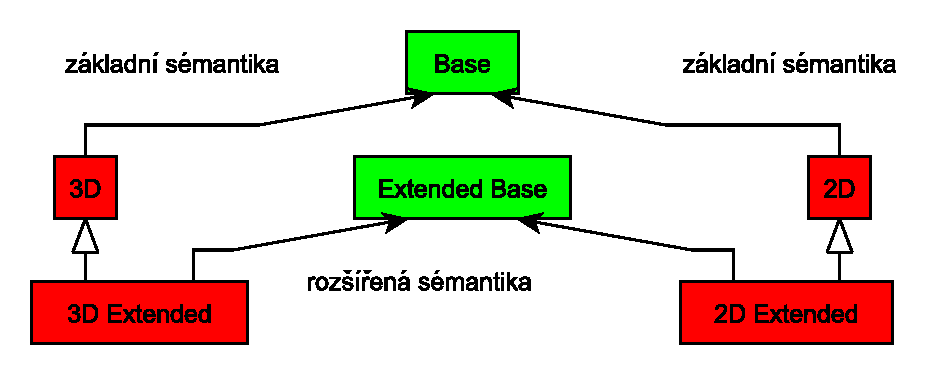
\includegraphics[width=0.8\linewidth]{pics/BU_schemas.pdf} % <-- use this for your graphics
%\rule{10cm}{5cm} % <-- this is just a black box substitute for graphics
\caption{Application schemas of the theme Buildings.}
\label{fig:building_schemas}
\end{figure*}

According to the specification, two different feature types shall be implemented -- \textit{building} and \textit{building part}. Buildings are enclosed constructions above and/or underground which are intended or used for the shelter of humans, animals, things or the production of economic goods and that refer to any structure permanently constructed or erected on its site. (...) A BuildingPart is a sub-division of a Building that might have been considered as a building and that is homogeneous related to its physical, functional or temporal aspects. It is up to each data producer to define what is considered as a Building and what is considered as a BuildingPart (if this concept is used). \cite{INSPIRE:DSBU}

\subsection{Data content and structure}
\label{sec:content}

In the Data specification for the theme Buildings are defined six application schemas (\ref{fig:building_schemas}). Two of them contain only abstract feature types. It means, similar to object programming, that single feature cannot be an instance of abstract feature type. But another feature types can inherit attributes from them. These two abstract application schemas are called \textit{BuildingsBase} and \textit{BuildingsExtended} and contain basically all semantic information. Other four application schemas differ in the used type of geometry on 2D and 3D and in the abstract schema they inherit from. According to the geometry and semantic depth there are distinguished application schemas \textit{BuildingsCore2D}, \textit{BuildingsExtended2D}, \textit{BuildingsCore3D} and \textit{BuildingsExtended3D}. Before the decision, which application schema will be the best for use over the data from the resort of Czech Office for Surveying, Mapping and Cadastre (including data of Land Survey Office), it was necessary to analyse data sources.

Databases containing reference data on buildings are three: Information System of Cadastre of Real Estates (ISKN) and Information System of Territorial Identification (ISUI) managed by Czech Office for Surveying, Mapping and Cadastre and Fundamental Base of Geographic Data (ZABAGED \circledR) managed by Land Survey Office. Data of the first two systems refer to the legal status, data from ZABAGED refer to the status in terrain. Unfortunately, data in the databases are not properly connected among those two organisations. Data used for the creation of the series of datasets for the theme Buildings come from ISKN and ISUI. All data corresponding with the possible content of the theme Buildings has only 2D geometry. Most of the buildings are represented as a polygon of the intersection of the walls with ground. Some of them are represented only as reference points of the buildings, laying somewhere in the building body. Spatial objects to be represented as featureType \textit{building} were clear -- buildings itself. In the case of \textit{buildingParts} there were two options: data of buildings in ISKN have their parts as inner drawings, on the other hand, buildings in ISUI have their parts represented as entrances, where each entrance consists from technical and economical information, such as number of floors, dwellings, connection to the engineering networks, property value et cetera. From the given possibilities, as the most usable data for the implementation were considered data for buildings taken both from ISKN and ISUI with entrances from ISUI used as \textit{buildingParts}.

\begin{figure*}
\centering
\includegraphics[width=0.8\linewidth]{pics/bu_wms.png} % <-- use this for your graphics
%\rule{10cm}{5cm} % <-- this is just a black box substitute for graphics
\caption{Building and building parts shown with default style.}
\label{fig:bu_portrayal}
\end{figure*}

Due to the lack of three dimensional data, only two non--abstract application schemas are applicable -- \textit{ BuildingsCore2D} inhering from \textit{BuildingsBase} and \textit{BuildingsExtended2D}, which inherits from  \textit{BuildingsExtended}. Semantic model of \textit{BuildingsBase} is very flat. It contains four abstract feature types -- \textit{AbstractConstruction}, \textit{AbstractBuilding}, that inherits from \textit{AbstractConstruction}, \textit{Building} and \textit{BuildingPart}, inheriting from \textit{AbstractBuilding}. Only extension given to \textit{Building} is attribute \textit{parts}. Its content is reference to feature(s) of the type \textit{BuildingPart}. Semantic information about construction given by the feature type \textit{AbstractCOnstruction} from the application schema \textit{BuildingsBase} are few: obligatory Inspire Id and voidable information about life cycle of feature, dates of construction/demolition/renovation, condition, elevation, name and height above ground of the construction and external reference on the spatial object in another register, such cadastral viewer. Feature type \textit{AbstractBuilding} extends semantic information on  building nature, current use and numbers of dwellings, building units and floors. As mentioned in previous paragraph, source databases contain much more detailed information about buildings and their parts. Besides technical economic information, there are links to other spatial objects, such as cadastral parcel on which is the building constructed or delivery points belonging to the building in the source databases as well. In the scope of the implementation of INSPIRE, parcels, municipalities and address points were already implemented (in the scope of INSPIRE themes Cadastral Parcels, Administrative Units and Addresses). Information about connections between features form various series of datasets is one of the biggest advantages of INSPIRE. Therefore it is really important to have links connecting buildings with other features. Otherwise, publication of the theme Building following application schema \textit{BuildingsCore2D} has no benefits compared to national products published upon data based on same source databases other than standardised structure. According to the previous analysis, it was decided to transform data according to the application schema \textit{BuildingsExtended2D}. 

As said before (\ref{sec:analysis}), application schemas contain structured information about data content and structure in the text form. But data itself shall be published in the GML 3.2.1 format, which is format standardised by Open Geospatial Consortium (OGC \cite{OGC:GML}). Validity of data content and structure is ensured by validation against XSD schemas. Joint Research Center publishes XSD schemas for INSPIRE application schemas on the web page \url{http://inspire.ec.europa.eu/schemas/}. For the theme Buildings, only three application schemas have their corresponding XSD schemas already published. Unfortunately, \textit{BuildingsExtended}, \textit{BuidlingsExtended2D} and \textit{BuidlingsExtended3D} are missing. At the end of 2014, after correspondence with Michael Lutz, JRCs Technical / data modelling contact point for INSPIRE data specifications, it was clear, that JRC is not creating XSD schemas for BuildingsExtended application schmeas in the near future. Publication of buildings according to other application schema then \textit{BuildingsExtended2D} was pointless. Therefore it was necessary to write XSD schemas for the application schemas \textit{BuildingsExtended} and \textit{BuildingsExtended2D} on my own.

Some other problems have appeared in the feature catalogue. In the application schema \textit{BuildingsExtended2D}, there are two attributes used for the number of floors. One of them shall contain number of floors above ground, second one only the number of floors bellow ground. In the source databases for the implementation of the theme Buildings in the Czech Republic, there is only one information about building floors, that sums up all floors (above ground and below ground) together. Some other problems were found in code lists for used materials, current use of buildings or building nature. Code list values used in ISUI are quite difficult to pair with values from INSPIRE code lists. Some of them were transformed into INSPIRE values, some were left empty. In the future it could be fixed on the side of transformation between ISUI and INSPIRE compliant data. All the information mediated by problematic code lists are voidable, according to the Data specification on Buildings. Problems and issues on INSPIRE theme Buildings (and other themes related to topography or cadastre) are reported and discussed in INSPIRE Thematic Clusters (\url{http://themes.jrc.ec.europa.eu/groups/profile/209/topographic-and-cadastral-reference-data}).

\subsection{Portrayal}
\label{sec:portrayal}

Chapter "Portrayal" in the Data specification defines rules for layers and styles to be used for portrayal of the spatial objects defined in Specification. These rules are used during implementation of INSPIRE View Services according to the Technical Guidance for the implementation of INSPIRE View Services in the version 3.11 of 4th April 2013 (\url{http://inspire.ec.europa.eu/documents/Network_Services/TechnicalGuidance_ViewServices_v3.11.pdf}). Basically, this guidance shows how to implement view services using OGC standard for Web Map Service in version 1.3.0 according to ISO 19128 and/or Web Map Tile Service in version 1.0.0. Guidance describes mandatory and optional operations required for the implementation of INSPIRE--compliant View services. Chapter "Portrayal" defines the human-- and machine--readable names of layers and its default style. Default INSPIRE style shall be available in the service, but any additional national style can be defined as well.

\begin{table}
\centering
\begin{tabular}{lll}
\toprule\\
\bfseries Layer Name & \bfseries Layer Title & \bfseries Feature Type(s)
\\\Midrule
BU.Building & Building & Building
\\\midrule
BU.BuildingPart & BuildingPart & BuildingPart
\\\bottomrule
\end{tabular}
\caption{Layers defined for Portrayal.}
\label{tab:layers}
\end{table}

Layers defined for the view service for the INSPIRE theme Buildings are shown in the table \ref{tab:layers}. For the theme Buildings, only 2D styles are defined. Originally it is caused by the lack of SLD for 3D data \cite{INSPIRE:DSBU}. For the implementation of Buildings in the Czech Republic it is irrelevant at the moment, because there are no 3D data available.

\begin{figure*}
\centering
\includegraphics[width=0.8\linewidth]{pics/Buildings.png} % <-- use this for your graphics
%\rule{10cm}{5cm} % <-- this is just a black box substitute for graphics
\caption{The whole model of featureTypes of application schemas \textit{BuildingsBase}, \textit{BuildingsCore2D}, \textit{BuildingsExtended} and \textit{BuildingsExtended2D}.}
\label{fig:bu_features}
\end{figure*}

Each layer has defined default style. Style for both layers counts with two types of geometric representation. Building can be represented as polygon or definition point. Building part is represented by border lines or by definition point. Building as a polygon is represented as solid gray with black outline. Definition point of building is shown as solid dark gray point without any outline. Colour difference between point and polygon filling is clearly visible. Surface style for building part is hollow with solid black outline. On the other hand, point geometry for building parts is solid grey circle without any outline. It has the same colour as the filling of polygon in the case of surface geometry for building. Simply said, building parts aren't visible upon the buildings layer. As seen in the picture \ref{fig:bu_portrayal} on the building in north--eatern corner, building parts points are visible only when they crosses the outline of buildings polygons. Short--term solution is to define own style, in which building part point would have different colour than building polygon. Long--term solution lays in the hands of JRC and it is the official change of style in INSPIRE Data specification. This problem was also reported to the INSPIRE Thematic Clusters.

\section{Designing and extending INSPIRE schemas}
\label{sec:extending}

The main findings of the Data specification analysis are lack of XSD schemas for extended application schemas, expected source of data to use for the implementation and an unfortunate choice of layer styles. The only problem not enabling the implementation is the lack of XSD schemas and it is the main object of work described in this paper. It had to be created two application schemas -- one for abstract application schema \textit{BuidlingsExtendedBase} and one for \textit{BuildingsExtended2D}, inheriting form the previous one. This work was supported by the Grant Agency of the Czech Technical University in Prague, grant No. SGS15/056/OHK1/1T/11.

% about XSD
Definition of XML Schema Definition Language (XSD) according to its standard is language, which offers facilities for describing the structure and constraining the contents of XML documents, including those which exploit the XML Namespace facility. The schema language, which is itself represented in an XML vocabulary and uses namespaces, substantially reconstructs and considerably extends the capabilities found in XML document type definitions (DTDs). Its purpose is to define and describe a class of XML documents by using schema components to constrain and document the meaning, usage and relationships of their constituent parts: datatypes, elements and their content and attributes and their values. Schemas can also provide for the specification of additional document information, such as normalization and defaulting of attribute and element values. Schemas have facilities for self-documentation. \cite{XSD}

% about used software
File in XSD format is XML file as well and therefore it is suitable to use professional software for editing and creation of XML files. Author have personal experience with software oXygen by the company Syncro Soft SRL. For the creation of XSD files, there is specialised programme named oXygen XML Developer. This programme contains tools allowing better work with XSD schemas, including schema designer and XSLT editor and debugger. According to the future plans of work in next few years, XSLT transformations are going to be also very useful. 

% modelling
\subsection{Schema modelling}
\label{sec:modelling}

\begin{figure*}
\centering
\includegraphics[width=0.8\linewidth]{pics/BU_dedicnost_info.png} % <-- use this for your graphics
%\rule{10cm}{5cm} % <-- this is just a black box substitute for graphics
\caption{\textit{Building} element from the XSD schema \textit{BuildingsExtended2D} shown in the design mode of the software oXygen Developer.}
\label{fig:bu_building_element_oxy}
\end{figure*}

Two XSD schemas were designed in order to fulfil application schemas for the implementation of Buildings with 2D geometry and extended semantics. These schemas inherits a lot from feature types defined in \textit{BuildingsCore2D} and \textit{BuildingsBase}. All relations are visible in the picture \ref{fig:bu_features}. 

In the XSD schema design, few basic components are used: \texttt{elements}, \texttt{complex types}, \texttt{simple types} and \texttt{attributes}. They can be put together in \texttt{groups} or \texttt{attribute groups}. To define relations between them, compositors and wildcards are used. Compositors are used for creating content of complex types by other elements, different types of compositors define different relations between those elements. Wildcards serves as any element, respectively any attribute and it is used mainly in abstract elements. Finally there are directives \texttt{import}, \texttt{include }and \texttt{redefine} for using and extending elements from other XSD schemas. Feature types in XSD schemas \textit{BuildingsExtendedBase} and \textit{buildingsExtended2D} are represented by \texttt{complex type} elements. Most of the relations creating their content are \texttt{sequence} compositors. Every element has annotations, containing name and definition of the element. Every element has a given type, that shall be present in the current or imported XSD file. \texttt{Complex types} can include compositors such as \texttt{sequence}, that allow other elements to be used as a content.  In the picture \ref{fig:bu_building_element_oxy} there is element \textit{Building} with annotation and defined \texttt{complex type} containing \texttt{sequence} compositor, that extends content by another element (\textit{buildingInfo}).

Designing the XSD schema begun with importing inherited XSD schemas and defining their namespaces. Among imported schemas are also schemas needed for using some attributes, such as BaseTypes, GML or GMD, but also INSPIRE Addresses, Cadastral Parcels and Geographical Names. It is much better to use a data type, that is already designed in another schema, as an attribute type, than create a new one. In the picture \ref{fig:bu_features} is possible to see abstract feature types \textit{AbstractOtherConstruction}, \textit{AbstractInstallation}  and \textit{AbstractBuildingUnit} and \textit{OtherConstruction}, \textit{Installation} and \textit{BuildingUnit} inheriting from them. These feature types aren't use in the Czech imlementation of the theme Buildings, but are included in the XSD schema as well. There was an intent to design XSD schemas as close to the application schemas described in the data specification document, including feature types not intended to use in the implementation itself.

The most important feature types for the implementation are \textit{Building }and \textit{BuildingPart }from the application schema \textit{BuildingsExtended2D}. They inherit both from \textit{BuildingInfo} and homonymous feature type from the application schema \textit{BuildingsCore2D}. Technically it's not really possible for one feature type to inherit from more than one another feature type. All semantic information given by the base application schemas and geometry representation are inherited from the \textit{Building} (respectively \textit{BuildingPart}) feature type, extended semantics shall be inherited from the \textit{BuildingInfo} feature type, that is abstract. The solution of the problem with multiple inheritance was solved by creating an instance of \textit{BuildingInfo} and creating the new attribute of the \textit{Building }feature type, that contains this instance of \textit{BuildingInfo}. It is not possible to create instances of the abstract feature types,  therefore it was necessary to design new feature type \textit{BuildingInfo} in the XSD schema \textit{BuildingsExtended2D}, that inherits from the feature type \textit{BuildingInfo} from the \textit{BuildingsExtendedBase} schema, but is not abstract. 

% use by JRC 
According to the latest information from JRC, newly created XSD schemas described in this paper are currently tested to be used as official XSD schemas for application schemas \textit{BuildingsExtendedBase} and \textit{BuildingsExtended2D}\footnote{it was said by Robert Tomas at the international conference INSPIRUJME SE... 2015, which was held 24th and 25th of November 2015 in Bratislava, Slovakia}. 

\begin{figure*}
\centering
\includegraphics[width=0.8\linewidth]{pics/BU_PUBL_DB.pdf} % <-- use this for your graphics
%\rule{10cm}{5cm} % <-- this is just a black box substitute for graphics
\caption{Schema of tables of the publication database related to the Buildings theme.}
\label{fig:publication_db}
\end{figure*}

\section{Publication of INSPIRE data}
\label{sec:publication}

The whole process of the implementation shall escalate with publication of data according to the Commission Regulations No 976/2009 of 19th October 2009 and 1311/2014 of 10th December 2014, amending Regulation No 976/2009. Ways of the publication are described in detail in the Technical Guidance documents for the implementation of INSPIRE Network services, for the data publication concretely Download Services and figuratively View Services \cite{INSPIRE:NS}. Process of the publication consists of the three stages -- data transformation, setting up services and creation of metadata.

\subsection{Transformation process}

\begin{figure}
\centering
\includegraphics[width=0.8\linewidth]{pics/transformace.png} % <-- use this for your graphics
%\rule{10cm}{5cm} % <-- this is just a black box substitute for graphics
\caption{Schema of the transformation process of data.}
\label{fig:transformation}
\end{figure}

In the beginning, data are stored in source database(s). These databases usually have their own structure, which is useful for its purpose. Purpose of INSPIRE compliant datasets could be different. Data transformation process therefore have more stages of transformations \ref{fig:transformation}. At first, data from source databases have to be transformed into publication database. In tables of this database, data structure basically respects the structure of source databases \ref{fig:publication_db}. There are few more tables ensuring the interoperability of the data from two (or more) databases. For the purpose of the data publication, database views are created in the publication database. Views are using data from the tables in the source structure, putting them into the INSPIRE structure, more or less following INSPIRE application and XSD schemas. From the database views, data are transformed on the fly into GML format in the structure valid against XSD schemas. An exception is publication of pre--defined data files (one for each municipality). These files are generated daily and they are valid to the early morning of each day (all changes are published next day in the early morning).

In the first stage of transformation, the biggest problem was to unify identifiers of the buildings and their parts from different databases. As seen in the picture \ref{fig:publication_db}, table PUB\_mustek was created. Attribute \texttt{Id} in this table is automatically generated from the sequence and is further used as a unique INSPIRE feature identifier. Connecting the data through this identifier allows merging information about one building from different databases. In the ISKN database, there is basically better information about geometry and it contains link to cadastral parcel, on the other hand, in the ISUI database are much more detailed informations about semantics and there is also connection to address, as an attribute of building part. 

During creation of database views, it was important to decide, which source of information is more relevant in the case, when both databases provide different value for the same attribute. This can happen in the case of geometry, link to municipality or part of municipality and buildings current use. The most often case is multiple geometry. The first choice of geometry is polygonal geometry coming from ISKN,  than it is point geometry from ISUI and the last choice is using point geometry coming from ISKN. In many cases ISUI also contains polygonal geometry, but it is always taken from ISKN, that is preferable. There are two main database views created for the publication of feature types -- Buildings and BuildingParts -- and few more for the complex types used in the GML structure, such as ExternalReference or BuildingGeometry2D. Names of the attributes in the database views are the same like the names of GML attributes.

Data structures are given by XSD schemas, but content depends on the local data as well. For the purpose of investigating possibilities, sample files were created. Every sample file tries to cover one of the possibilities. Samples vary in the geometry type and source or number of building parts belonging to the building. More in \cite{Med15:230877} (in czech language). With the samples come out a need of converting national code lists into INSPIRE code lists as well. For every code list is created new converter table in the publication database. According to the latest version of sample file, third step of transformation is done.

The third step of the transformation transforms data from publication database into GML form. There are to cases in which is this transformation invoked. It coheres with the ways of publication of the data -- data are published either through the direct access or as pre--defined files. Pre--defined files are generated daily for the predetermined area. For the theme Buildings, every file contains all features in the area of a single municipality. These files are generated every day in the early morning hours. Direct access via Web Feature Service provides recent data (no more than two hours old), but every single request comes straight into database. These two mods are recommended by the Technical Guidance for the implementation of INSPIRE Download Service in the version 3.1 \cite{INSPIRE:DLS}. 

\subsection{Services}

Two kinds of services are required for the publication of INSPIRE data -- Download Services and View Services. Two more services are considered as the INSPIRE Network Services. Discovery Service is used for searching in the metadata records of data and services present in the metadata catalogue, Transformation Services are used to transformation of schemas and coordinates \cite{INSPIRE:NS}.

Access to the data is allowed by Download service. Technical Guidance for the implementation of Download Services contains set of recommendations and requirements referencing standards ISO 19142, ISO 19143 and/or standard for ATOM. ISO standards describe the use and conformance classes of the Web Feature Service as defined in the OGC standard \cite{OGC:WFS}. The basic requirements of INSPIRE compliant service are publication of pre--defined datasets via either ATOM or WFS and direct access download service using WFS. Quality of the INSPIRE Download Services provided by Czech Office for Surveying, Mapping and Cadastre were tested by the Technical University of Ostrava\cite{Horak:geoinformatics10}.

Another service used for the access to the data is View service, but user doesn't get the raw data, only it's image. Technical Guidance for the implementation of View Services uses references to the standard ISO 19128, refering to the Web Map Service as defined in the OGC standard\cite{OGC:WMS}. The minimum requirements of the INSPIRE service is the usage of operations GetMap and GetCapabalities. GetCapabilities shall be extended according to the Technical Guidance.

\subsection{Metadata}

Without the information about the data, data itself are useless. Therefore they have to be provided with the metadata records. The metadata shall contain information about the origin of the data, about data provider, quality and its date and shall be consistent to the standard ISO 19115. Services shall be provided with metadata as well. Authoritative document for the services metadata is standard ISO 19119. All INSPIRE recommendations and requirements on both data and services metadata can be found in the INSPIRE Metadata Implementing Rules: Technical Guidelines based on EN ISO 19115 and EN ISO 19119 \cite{INSPIRE:MD}. In the Czech Republic, standard ISO 19115 is widely used, but ISO 19115 conformance itself does not mean, that metadata are INSPIRE--compatible\cite{Ruzicka:geoinformatics3}. In the Czech Republic, there is National Metadata Catalogue, managed and published by Technical Working Group for Metadata, established under the Coordinating Committee for INSPIRE (KOVIN). This metadata Catalogue fully covers INSPIRE requirements on metadata. Some organisations (e.g. Czech Office for Surveying, Mapping and Cadastre) have their own Metadata Profiles, extending National Matadata Profile.

Consistency of metadata records can be checked in the INSPIRE matadata validator, accessible through the INSPIRE geoportal \cite{INSPIRE:GP}. This validator is very complex and reflects not only metadata conformity, but quality and requirements for services as well. 

\section{Conclusions}

After the analysis of the Data specification on Buildings in the version 3.0 from the 10th December 2013, it has shown up, that for the meaningful implementation of the INSPIRE theme Buildings, it is necessary to create XSD schemas following application schemas \textit{BuildingsExtendedBase} and \textit{BuildingsExtended2D}.

During designing the schemas, some problems have appeared. Application schema expected multiple inheritance for feature types \texttt{Building} and \texttt{BuildingPart}, that is not possible to easily and effectively design. Therefore it has to be solved another way, that doesn't correspond to the application schema. 

Source data for the implementation of the theme Buildings in the Czech Republic are stored in three databases -- ISKN, ISUI and ZABAGED\circledR. The last one mentioned has no links to others. Data from the source databases are transformed into publication database and according to the sample file, they are transformed into the GML format.


\begin{acknowledgements}
This work was supported by the Grant Agency of the Czech Technical University in Prague, grant No. SGS15/056/OHK1/1T/11.\end{acknowledgements}


\bibliographystyle{actapoly}
\bibliography{biblio}

\nocite{Med13:Geoinformatics11} % uvede necitovaný zdroj
\nocite{Tryhubova13:geoinformatics1}
\nocite{Polacek:geoinformatics8}

\end{document}
